% CVPR 2026 Paper Template; see https://github.com/cvpr-org/author-kit

\documentclass[10pt,twocolumn,letterpaper]{article}

%%%%%%%%% PAPER TYPE  - PLEASE UPDATE FOR FINAL VERSION
% \usepackage{cvpr}              % To produce the CAMERA-READY version (non-anonymous)
\usepackage[review]{cvpr}      % To produce the REVIEW version (anonymous, required for double-blind submission)
% \usepackage[pagenumbers]{cvpr} % To force page numbers, e.g. for an arXiv version

% Import additional packages in the preamble file, before hyperref
%% This file contains a number of tweaks that are typically applied to the main document.
%% They are not enabled by default, but can be enabled by uncommenting the relevant lines.

\usepackage{float}
\WarningFilter{caption}{Unused}
\usepackage{graphicx}
\usepackage{multirow}
\usepackage[most]{tcolorbox}
\usepackage{amssymb}
\usepackage[table]{xcolor}

% tcolorbox colors (matching NeurIPS-2026-Position style)
\definecolor{mainquestionbg}{RGB}{255, 245, 245} % Light red for background
\definecolor{mainquestionframe}{RGB}{200, 80, 80}  % Lighter red for frame
\usepackage{subcaption}
\usepackage{enumitem}
\usepackage{bm}

%%
%% Inline annotations; for predefined colors, refer to "dvipsnames" in the xcolor package:
%% https://tinyurl.com/overleaf-colors
%%
\newcommand{\red}[1]{{\color{red}#1}}
\newcommand{\todo}[1]{{\color{red}#1}}
\newcommand{\TODO}[1]{\textbf{\color{red}[TODO: #1]}}
%%
%% disable for camera ready / submission by uncommenting these lines  
%%
% \renewcommand{\TODO}[1]{}
% \renewcommand{\todo}[1]{#1}

%%
%% work harder in optimizing text layout. Typically shrinks text by 1/6 of page, enable
%% it at the very end of the writing process, when you are just above the page limit
%%
% \usepackage{microtype}

%%
%% fine-tune paragraph spacing
%%
% \renewcommand{\paragraph}[1]{\vspace{.5em}\noindent\textbf{#1.}}

%%
%% globally adjusts space between figure and caption
%%
% \setlength{\abovecaptionskip}{.5em}


%%
%% Allows "the use of \paper to refer to the project name"
%% with automatic management of space at the end of the word
%%
% \usepackage{xspace}
% \newcommand{\paper}{ProjectName\xspace}

%%
%% Commonly used math definitions
%%
% \DeclareMathOperator*{\argmin}{arg\,min}
% \DeclareMathOperator*{\argmax}{arg\,max}

%%
%% Tigthen underline
%%
% \usepackage{soul}
% \setuldepth{foobar}


% It is strongly recommended to use hyperref, especially for the review version.
% hyperref with option pagebackref eases the reviewers' job.
% Please disable hyperref *only* if you encounter grave issues, 
% e.g. with the file validation for the camera-ready version.
%
% If you comment hyperref and then uncomment it, you should delete *.aux before re-running LaTeX.
% (Or just hit 'q' on the first LaTeX run, let it finish, and you should be clear).
\definecolor{cvprblue}{rgb}{0.21,0.49,0.74}
\usepackage[pagebackref,breaklinks,colorlinks,allcolors=cvprblue]{hyperref}

% Teaser figure configuration
\makeatletter
\apptocmd{\@maketitle}{%
  \vspace{-1em}
\begin{center}
    \centering
    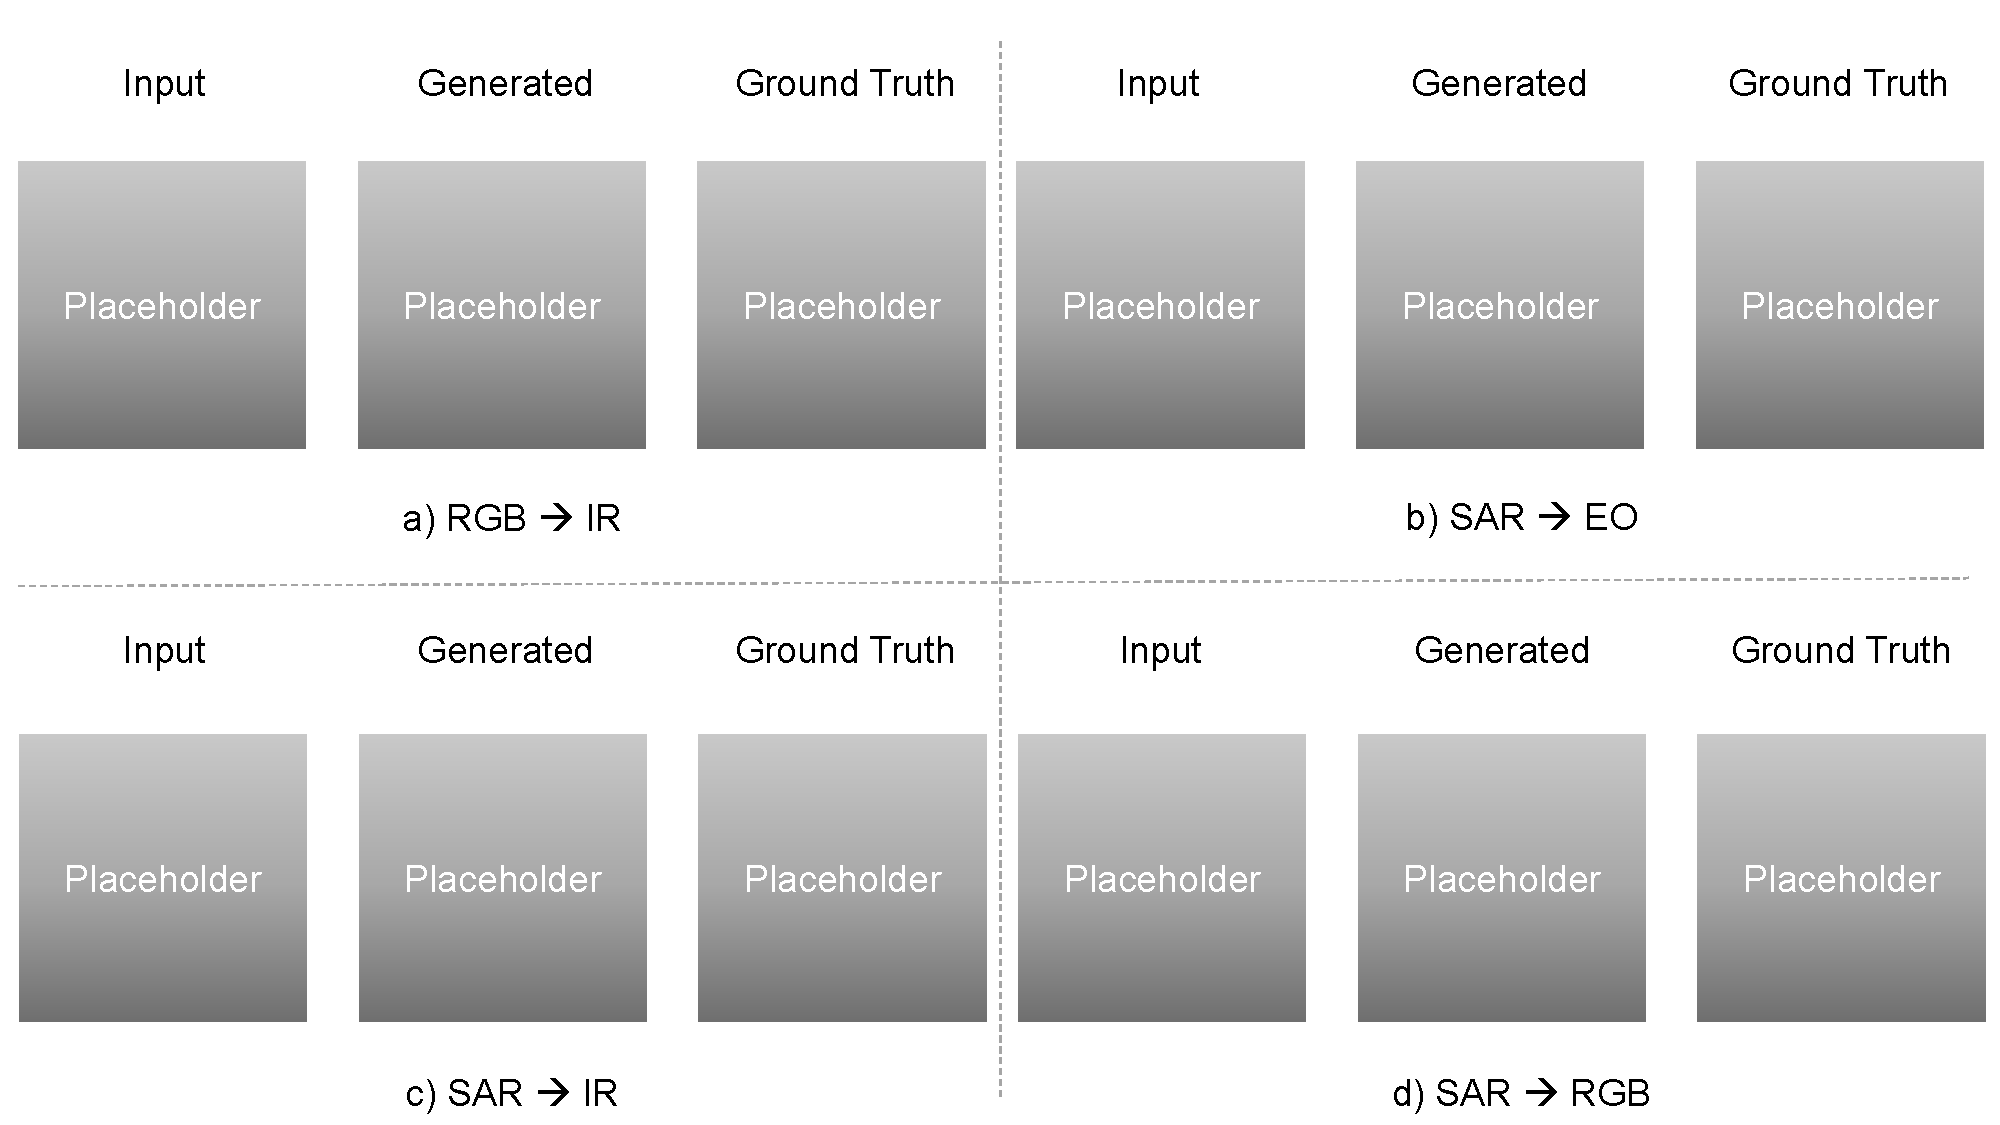
\includegraphics[page=1,width=0.95\textwidth]{figures/Figures.pdf}
    \captionof{figure}{Teaser: The proposed EarthBridge framework for multi-modal aerial-view image translation across Electro-Optical (EO), Infrared (IR), and Synthetic Aperture Radar (SAR) modalities. Our method accurately bridges the domain gap, preserving structural integrity while synthesizing high-fidelity target textures.}
    \label{fig:teaser}
\end{center}
  \vspace{1em}
}{}{}
\makeatother

%%%%%%%%% PAPER ID  - PLEASE UPDATE
\def\paperID{*****} % *** Enter the Paper ID here
\def\confName{CVPR}
\def\confYear{2026}

%%%%%%%%% TITLE - PLEASE UPDATE
\title{EarthBridge: A Solution for 4th Multi-modal Aerial View Image Challenge Translation Track}

%%%%%%%%% AUTHORS - PLEASE UPDATE
\author{Zhenyuan Chen$^\dagger$\\
Zhejiang University\\
% School of Earth Sciences\\
{\tt\small bili_sakura@zju.edu.cn}
\and
Yuanshen Guan$^\dagger$\\
University of Science and Technology of China\\
{\tt\small guanys@mail.ustc.edu.cn}
\and
Feng Zhang\\
Zhejiang University\\
% School of Earth Sciences\\
{\tt\small zfcarnation@zju.edu.cn}
}

\begin{document}

\maketitle

\begin{abstract}
This paper presents our solution for the 4th Multi-modal Aerial View Image Challenge - Translation (4th-MAVIC-T), submitted to the PBVS workshop at \confName~\confYear. The challenge focuses on multi-modal image translation between SAR, EO, IR, and RGB imagery to enable high-quality and high-fidelity cross-modal image generation. Our approach addresses the domain translation problem by leveraging recent advances in remote sensing image-to-image translation, building upon GAN-based methods and diffusion models for SAR-to-optical translation. We reference the 3rd Multi-modal Aerial View Image Challenge \citep{bowald3rdMultimodalAerial2025} as a foundation for this work.
\end{abstract}    

\section{Introduction}
\label{sec:intro}



The Multi-modal Aerial View Image Challenge for cross domain image translation~\cite{lowMultimodalAerialView2024,lowMultimodalAerialView2023,bowald3rdMultimodalAerial2025} is a leading challenge held in conjunction with the Perception Beyond the Visible Spectrum (PBVS) workshop from 2023 to 2025. Data collected across multiple sensing modalities---such as Electro-Optical (EO), Infrared (IR), and Synthetic Aperture Radar (SAR)---each capture distinct characteristics and measurements of objects, providing complementary perspectives on the same scene. However, data coverage limitations and modality-specific constraints often hinder the full utilization of these diverse sources. For instance, while SAR sensors offer all-weather capabilities and can penetrate atmospheric obstructions, their imagery is complex to interpret and publicly available datasets are scarce. Conversely, widely available EO imagery is limited by lighting conditions and atmospheric visibility. Domain translation seeks to bridge this gap by converting one modality into another, enabling cross-modal data synthesis and enhancing sensor interoperability. By focusing on translation tasks such as RGB$\rightarrow$IR, SAR$\rightarrow$EO, SAR$\rightarrow$IR, and SAR$\rightarrow$RGB, the MAVIC-T challenge aims to bolster existing data volume, increase data diversity across regions, and serve as a platform for advancing conditioned image synthesis techniques, ultimately fostering the development of more adaptable and robust models for multi-modal image analysis.

% paragraph: talk about the difficulty to do image translation across above different modality (with proper work citation)
interpret SAR need special knowledge~\cite{majumder2020deep}.

% paragraph: our solution
In this paper, we propose [YourMethodName], a novel [Diffusion/GAN/Transformer] framework designed to [solve specific problem]. Our approach incorporates a [Specific Module, e.g., 'Latent Consistency Constraint'] and a [Specific Loss] to ensure that the translated images maintain the precise geometric layout of the source modality while achieving high photorealism.

% (optional) paragraph: Key Findings & Results
% Our findings indicate that [Specific Technique] significantly reduces the FID score by [X%]. Qualitatively, our model demonstrates a superior ability to reconstruct urban structures in SAR-to-RGB tasks compared to the baseline models provided in the challenge. Furthermore, our solution placed [Rank] in the [Task Name] leaderboard, proving its robustness across diverse geographical regions.

% paragraph: Contributions    
\section{Related Work}
\label{sec:related_work}

\paragraph{Image-to-Image Translation.}
Image-to-image translation has been extensively studied in computer vision. Foundational works include Pix2Pix for paired conditional translation~\cite{isolaImageToImageTranslationConditional2017} and CycleGAN for unpaired translation~\cite{zhuUnpairedImageToImageTranslation2017}. Subsequent advances include contrastive learning for unpaired translation~\cite{parkContrastiveLearningUnpaired2020}, zero-shot~\cite{parmarZeroshotImagetoImageTranslation2023} and one-step translation with text-to-image models~\cite{parmarOneStepImageTranslation2024}.

\paragraph{Diffusion Bridge Models.}
Unlike standard diffusion models that generate from noise, diffusion bridge models learn a stochastic process that directly connects source and target distributions, making them well-suited for paired image-to-image translation. Denoising Diffusion Bridge Models (DDBM)~\cite{zhouDenoisingDiffusionBridge2024} define a variance-preserving bridge between data distributions. Related formulations include Brownian Bridge Diffusion Models (BBDM)~\cite{Li_2023_CVPR} and its bidirectional extension BiBBDM~\cite{xueBiBBDMBidirectionalImage2025}, Image-to-Image Schr\"odinger Bridge (I$^2$SB)~\cite{liuI2SBImagetoImageSchrodinger2023}, Diffusion Schr\"odinger Bridge matching~\cite{shiDiffusionSchrodingerBridge2023}, Dual Diffusion Implicit Bridges~\cite{suDualDiffusionImplicit2023a}, and Direct Diffusion Bridge with data consistency~\cite{chungDirectDiffusionBridge2023}. Recent extensions include Consistency Diffusion Bridge~\cite{heConsistencyDiffusionBridge2024}, Diffusion Bridge Implicit Models~\cite{zhengDiffusionBridgeImplicit2025}, deterministic translation via denoising Brownian bridge with dual approximators~\cite{xiaoDeterministicImagetoImageTranslation2025a}, and adaptive domain shift for cross-modality translation~\cite{wangAdaptiveDomainShift2026a}.

\paragraph{Cross-Modality Translation.}
Image translation across diverse sensor modalities---grayscale, near-infrared (NIR), thermal colorization, and color transfer---has been addressed with probabilistic color correction~\cite{oliveiraProbabilisticApproachColor2015}, NIR imagery colorization~\cite{suarezInfraRedImageryColorization2018}, deep colorization~\cite{zhangColorfulImageColorization2016,majumder2020deep}. Our work extends diffusion bridge models to cross-modal remote sensing translation across EO, IR, and SAR modalities in the MAVIC-T challenge setting.

\section{Preliminary}
\label{sec:preliminary}

\paragraph{Problem Formulation}
Let $\mathcal{X} \subset \mathbb{R}^{C_s \times H \times W}$ denote the source domain and $\mathcal{Y} \subset \mathbb{R}^{C_t \times H \times W}$ denote the target domain, where $C_s$ and $C_t$ are the number of channels in the source and target modalities, respectively. Given a set of spatially-aligned training pairs $\{(x_i, y_i)\}_{i=1}^{N}$ with $x_i \in \mathcal{X}$ and $y_i \in \mathcal{Y}$, the goal of cross-modal image-to-image translation is to learn a mapping $G: \mathcal{X} \rightarrow \mathcal{Y}$ that minimizes a composite distance between the generated image $\hat{y} = G(x)$ and the ground-truth target $y$. In the context of the MAVIC-T challenge, four translation tasks are defined: SAR$\rightarrow$EO ($1 \!\rightarrow\! 1$ channel, $256 \times 256$), SAR$\rightarrow$RGB ($1 \!\rightarrow\! 3$, $1024 \times 1024$), SAR$\rightarrow$IR ($1 \!\rightarrow\! 1$, $1024 \times 1024$), and RGB$\rightarrow$IR ($3 \!\rightarrow\! 1$, $1024 \times 1024$).

\begin{table}[H]
\centering
\caption{Task specifications for the MAVIC-T challenge.}
\label{tab:task_specs}
\resizebox{\columnwidth}{!}{%
\begin{tabular}{lccc}
\toprule
Task & Modality Mapping & Resolution & Channels \\
\midrule
SAR$\rightarrow$EO & SAR $\rightarrow$ Electro-Optical & $256^2$ & $1 \rightarrow 1$ \\
SAR$\rightarrow$RGB & SAR $\rightarrow$ RGB & $1024^2$ & $1 \rightarrow 3$ \\
SAR$\rightarrow$IR & SAR $\rightarrow$ Infrared & $1024^2$ & $1 \rightarrow 1$ \\
RGB$\rightarrow$IR & RGB $\rightarrow$ Infrared & $1024^2$ & $3 \rightarrow 1$ \\
\bottomrule
\end{tabular}
}
\end{table}

\paragraph{Evaluation Metric}
The MAVIC-T challenge evaluates submissions using a composite score derived from three complementary metrics: LPIPS~\cite{zhangUnreasonableEffectivenessDeep2018} (Learned Perceptual Image Patch Similarity, based on VGG-16) for perceptual fidelity, FID~\cite{heuselGANsTrainedTwo2017} (Fr\'{e}chet Inception Distance, based on InceptionV3) for distributional similarity, and L1 norm for pixel-level structural accuracy. These are combined into a task score:
\begin{equation}
    S_{\text{task}} = \frac{\tfrac{2}{\pi}\arctan(\text{FID}) + \text{LPIPS} + \text{L1}}{3}\,,
    \label{eq:task_score}
\end{equation}
where the $\arctan$ normalization maps FID into the $[0, 1]$ range to balance its contribution against the other two metrics. The overall score is the average of the four task scores, with a penalty of $+1$ added for each unattempted domain, encouraging participants to develop generalizable solutions across all modality pairs.
% }

% }

% Proposed Method (2.5 pages): This is the "meat." Use a high-quality system diagram. Break it down into:
% Problem Formulation: Mathematical definition of the translation tasks.
% Architecture: Specifics of your model (e.g., UNet, Transformers).
% Loss Functions: What drives the learning (adversarial, perceptual, cycle-consistency).
% Experiments (2 pages):
% Experimental Setup: Dataset splits and implementation details.
% Quantitative Results: Tables showing you outperformed baselines or previous years.
% Qualitative Results: High-res visual comparisons (SAR vs. Synthetic EO vs. Real EO).
% Ablation Study: Show that each part of your method actually helps.
\section{Lessons and Insights}
\label{sec:lessons}

We summarize key lessons and insights from developing EarthBridge for the MAVIC-T translation track.

\section{Conclusion}
\label{sec:conclusion}

In this paper, we presented EarthBridge, a novel solution for the 4th Multi-modal Aerial View Image Challenge -- Translation (MAVIC-T). By leveraging Diffusion Bridge Implicit Models (DBIM), we generalized the diffusion bridge framework with non-Markovian processes, enabling efficient and deterministic cross-modal translation. Our approach effectively handles disparate sensor characteristics across EO, IR, and SAR modalities through pixel-level modeling and a specialized training protocol featuring Karras-weighted bridge scalings. Quantitative and qualitative evaluations across four translation tasks demonstrate EarthBridge's superior ability to preserve spatial structure while generating high-fidelity target textures. Future work will explore the integration of adaptive domain shift mechanisms and further optimization for real-time remote sensing applications. \TODO{Add final ranking and summary of key findings.}

\clearpage
{
    % \small
    % \setlength{\bibsep}{0pt}
    % \setlength{\itemsep}{0pt}
    \setlength{\parskip}{0pt}
    \bibliographystyle{ieeenat_fullname}
    \bibliography{main}
}

% WARNING: do not forget to delete the supplementary pages from your submission 
\clearpage
\hypersetup{pageanchor=false}
\setcounter{page}{1}
\maketitlesupplementary


\section{Extended Related Work}
\label{sec:suppl_related_work}

This section provides a comprehensive literature review of image-to-image translation, diffusion bridge models, and cross-modality translation to complement the specialized discussion on remote sensing in the main paper.

\paragraph{General Image-to-Image Translation.}
Image-to-image translation has been extensively studied in computer vision. Foundational works include Pix2Pix for paired conditional translation~\cite{isolaImageToImageTranslationConditional2017} and CycleGAN for unpaired translation~\cite{zhuUnpairedImageToImageTranslation2017}. Subsequent advances include contrastive learning for unpaired translation~\cite{parkContrastiveLearningUnpaired2020}, zero-shot~\cite{parmarZeroshotImagetoImageTranslation2023} and one-step translation with text-to-image models~\cite{parmarOneStepImageTranslation2024}.

\paragraph{Diffusion Bridge Models.}
Unlike standard diffusion models that generate from noise, diffusion bridge models learn a stochastic process that directly connects source and target distributions, making them well-suited for paired image-to-image translation. Denoising Diffusion Bridge Models (DDBM)~\cite{zhouDenoisingDiffusionBridge2024} define a variance-preserving bridge between data distributions. Related formulations include Brownian Bridge Diffusion Models (BBDM)~\cite{Li_2023_CVPR} and its bidirectional extension BiBBDM~\cite{xueBiBBDMBidirectionalImage2025}, Image-to-Image Schr\"odinger Bridge (I$^2$SB)~\cite{liuI2SBImagetoImageSchrodinger2023}, Diffusion Schr\"odinger Bridge matching~\cite{shiDiffusionSchrodingerBridge2023}, Dual Diffusion Implicit Bridges~\cite{suDualDiffusionImplicit2023a}, and Direct Diffusion Bridge with data consistency~\cite{chungDirectDiffusionBridge2023}. Recent extensions include Consistency Diffusion Bridge~\cite{heConsistencyDiffusionBridge2024}, Diffusion Bridge Implicit Models~\cite{zhengDiffusionBridgeImplicit2025}, deterministic translation via denoising Brownian bridge with dual approximators~\cite{xiaoDeterministicImagetoImageTranslation2025a}, and adaptive domain shift for cross-modality translation~\cite{wangAdaptiveDomainShift2026a}.

\paragraph{Cross-Modality Translation.}
Image translation across diverse sensor modalities---grayscale, near-infrared (NIR), thermal colorization, and color transfer---has been addressed with probabilistic color correction~\cite{oliveiraProbabilisticApproachColor2015}, NIR imagery colorization~\cite{suarezInfraRedImageryColorization2018}, deep colorization~\cite{zhangColorfulImageColorization2016,majumder2020deep}. 

\paragraph{GAN-based RS Translation.}
Early attempts at translating between SAR and optical modalities leveraged Generative Adversarial Networks (GANs). For instance, Wang et al.~\cite{wangSARtoOpticalImageTranslation2022} proposed a hierarchical latent feature approach to improve the fidelity of SAR-to-optical translation. Hu et al.~\cite{huGanbasedSAROptical2022} specifically addressed this task in fire-disturbed regions using GANs to reconstruct optical details from SAR signals, which is vital for post-fire damage assessment when clouds or smoke obscure optical sensors.

\paragraph{Diffusion Models for RS Translation.}
Reflecting the recent shift in generative modeling, diffusion models have been increasingly applied to RS translation tasks. Qin et al.~\cite{qinConditionalDiffusionModel2024} introduced a conditional diffusion model incorporating spatial-frequency refinement to capture both global structure and fine-grained textures in SAR-to-optical translation. To address the computational overhead of iterative sampling, Qin et al.~\cite{qinEfficientEndtoEndDiffusion2025} later developed an efficient end-to-end diffusion model capable of one-step SAR-to-optical translation, significantly reducing inference latency while maintaining high generation quality. Furthermore, Wang et al.~\cite{wangAdaptiveDomainShift2026a} proposed adaptive domain shift mechanisms within diffusion frameworks to better handle the large distribution gaps inherent in cross-modality remote sensing datasets. These advancements underscore the growing role of stochastic bridge processes and diffusion-based refinement in enabling robust, high-resolution translation across heterogeneous sensor modalities.


\section{EarthBridge Architecture and Implementation Details}
\label{sec:suppl_architecture}

This section provides the comprehensive technical details of the EarthBridge architecture, training hyperparameters, and multi-modal refinement modules.

\subsection{UNet Denoising Backbone}
Our denoiser $D_\theta$ is implemented in PyTorch~\cite{paszkePyTorchImperativeStyle2019} and based on a \texttt{UNet2DModel} backbone from the Hugging Face Diffusers library~\cite{vonplatenDiffusersStateoftheartDiffusion2022} with Adaptive Group Normalization (ADM-style~\cite{dhariwalDiffusionModelsBeat2021}). The detailed architectural parameters are summarized in \cref{tab:suppl_unet_arch}.

\begin{table}[h]
\centering
\caption{{\color{gray}UNet denoising backbone architectural parameters.}}
\label{tab:suppl_unet_arch}
{\color{gray}
\resizebox{\columnwidth}{!}{%
\begin{tabular}{ll}
\toprule
Property & Details \\
\midrule
Backbone Type & UNet2DModel (ADM-style~\cite{dhariwalDiffusionModelsBeat2021}) \\
Normalization & Adaptive Group Normalization (AdaGN) \\
Base Channels & 128 \\
Channel Mult. & (1, 1, 2, 2, 4, 4) for $256\times256$ inputs \\
Block Channels & (128, 128, 256, 256, 512, 512) \\
Residual Blocks & 2 per resolution level \\
Self-Attention & Enabled at $32\times32$, $16\times16$, $8\times8$ resolutions \\
Attention Blocks & \texttt{AttnDownBlock2D}, \texttt{AttnUpBlock2D} \\
\bottomrule
\end{tabular}
}%
}
\end{table}

\subsection{Source Image Conditioning via Channel Concatenation}
To condition on the source image $\bm{x}$, we adopt a channel-concatenation strategy. The input configuration is summarized in \cref{tab:suppl_conditioning}.

\begin{table}[h]
\centering
\caption{{\color{gray}Source image conditioning configuration.}}
\label{tab:suppl_conditioning}
{\color{gray}
\resizebox{\columnwidth}{!}{%
\begin{tabular}{ll}
\toprule
Component & Configuration \\
\midrule
Strategy & Channel-wise concatenation $[\bm{z}_t, \bm{x}]$ \\
Input Channels & $2C$ ($C$ is target channel count) \\
Output Channels & $C$ (raw denoised prediction) \\
\bottomrule
\end{tabular}
}%
}
\end{table}

\subsection{Bridge Scalings and Schedules}
Following the Diffusion Bridge framework, the raw model output $F_\theta$ is post-processed through bridge scalings $(c_{\text{skip}}, c_{\text{out}}, c_{\text{in}})$ derived from the VP log-SNR schedule. The denoised prediction is defined as:
\begin{equation}
    D_\theta(\bm{z}_t, t, \bm{x}) = c_{\text{out}}(t) \cdot F_\theta(c_{\text{in}}(t) \cdot \bm{z}_t,\, t,\, \bm{x}) + c_{\text{skip}}(t) \cdot \bm{z}_t\,,
    \label{eq:suppl_denoiser}
\end{equation}
The scheduling and numerical parameters are summarized in \cref{tab:suppl_bridge_params}.

\begin{table}[h]
\centering
\caption{{\color{gray}Bridge scheduling and numerical parameters.}}
\label{tab:suppl_bridge_params}
{\color{gray}
\resizebox{\columnwidth}{!}{%
\begin{tabular}{ll}
\toprule
Parameter & Value \\
\midrule
VP schedule $\beta_d$ & $2.0$ \\
VP schedule $\beta_{\min}$ & $0.1$ \\
Numerical stability $\varepsilon$ & $10^{-44}$ \\
Timestep rescaling & $\hat{t} = 1000 \cdot 0.25 \cdot \log(\sigma + \varepsilon)$ \\
\bottomrule
\end{tabular}
}%
}
\end{table}

\subsection{Training Hyperparameters}
The primary training objective is a weighted mean squared error between the denoised prediction $D_\theta(\bm{z}_t, t, \bm{x})$ and the clean target $\bm{y}$:
\begin{equation}
    \mathcal{L}_{\text{denoise}} = \mathbb{E}_{(\bm{x},\bm{y}),\, t,\, \epsilon} \left[ w(t) \cdot \| D_\theta(\bm{z}_t, t, \bm{x}) - \bm{y} \|_2^2 \right],
    \label{eq:suppl_denoising_loss}
\end{equation}
where $w(t) = A(t) / c_{\text{out}}(t)^2$ is the Karras bridge weighting. The diffusion time $t$ is sampled from a Karras distribution with parameters in \cref{tab:suppl_train_params}.

\begin{table}[h]
\centering
\caption{{\color{gray}Training time-sampling parameters.}}
\label{tab:suppl_train_params}
{\color{gray}
\resizebox{\columnwidth}{!}{%
\begin{tabular}{ll}
\toprule
Parameter & Value \\
\midrule
Distribution & Karras inverse-$\rho$ \\
$\rho$ factor & $7$ \\
Sampling range & $[\sigma_{\min}, \sigma_{\max}]$ \\
Concentration & Low noise levels (fine details) \\
\bottomrule
\end{tabular}
}%
}
\end{table}


\section{Additional Implementation Details}
\label{sec:suppl_impl}

{\color{gray}
This section provides a summary of the implementation hyperparameters and training environment used for EarthBridge.

\begin{table}[h]
\centering
\caption{{\color{gray}Implementation hyperparameters and training environment.}}
\label{tab:suppl_impl_params}
{\color{gray}
\resizebox{\columnwidth}{!}{%
\begin{tabular}{ll}
\toprule
Category & Details \\
\midrule
Optimizer & Prodigy (adaptive, nominal $lr=1.0$) \\
LR Schedule & Constant with 500 warmup steps \\
Gradient Clipping & Max norm $1.0$ \\
Mixed Precision & bfloat16 (Hugging Face Accelerate) \\
EMA Decay & $0.9999$ (with warmup) \\
Model Format & Hugging Face Diffusers (safetensors) \\
Multi-GPU & Distributed via Accelerate (7200s timeout) \\
Gradient Accum. & 1 (default) \\
\bottomrule
\end{tabular}
}%
}
\end{table}
}


\section{Dataset Processing Details}
\label{sec:suppl_dataset}

{\color{gray}
The MAVIC-T dataset is a composite of three geospatial data sources with standardized preprocessing and chipping. Details of the dataset processing are summarized in \cref{tab:suppl_dataset}.

\begin{table}[h]
\centering
\caption{{\color{gray}MAVIC-T dataset processing and augmentation details.}}
\label{tab:suppl_dataset}
{\color{gray}
\resizebox{\columnwidth}{!}{%
\begin{tabular}{ll}
\toprule
Component & Details \\
\midrule
Data Sources & UNICORN, USGS EROS HRO, UMBRA SAR \\
Preprocessing & Georectification, alignment, GeoTIFF storage \\
Chip Size & 200m$\times$200m spatially aligned stacks \\
Geographic Scope & UC Davis, Manhattan, Bingham, Centerfield \\
Augmentation & Random crop/resize (for 1024px tasks) \\
Quality Filter & Skip manifest (\texttt{bad\_samples.txt}) \\
\bottomrule
\end{tabular}
}%
}
\end{table}
}


\section{Per-Task Configuration Summary}
\label{sec:suppl_config}

\begin{table}[h]
\centering
\caption{{\color{gray}Per-task EarthBridge configuration summary.}}
\label{tab:task_config_suppl}
{\color{gray}
\resizebox{\columnwidth}{!}{%
\begin{tabular}{lcccc}
\toprule
Parameter & SAR$\rightarrow$EO & SAR$\rightarrow$RGB & SAR$\rightarrow$IR & RGB$\rightarrow$IR \\
\midrule
Source channels     & 1   & 1   & 1   & 3   \\
Target channels     & 1   & 3   & 1   & 1   \\
Model channels      & 1   & 3   & 1   & 3   \\
Resolution          & 256 & 1024 & 1024 & 1024 \\
Batch size          & 32  & 8   & 8   & 8   \\
Crop augmentation   & No  & Yes & Yes & Yes \\
Inference steps     & 40  & 40  & 40  & 40  \\
\bottomrule
\end{tabular}
}%
}
\end{table}

{\color{gray}
\cref{tab:task_config_suppl} summarizes the per-task configuration for our EarthBridge method. All tasks share the same UNet backbone architecture (128 base channels, channel multipliers auto-detected from resolution), Prodigy optimizer (lr=1.0), EMA decay (0.9999), VP noise schedule ($\sigma_{\min}=0.002$, $\sigma_{\max}=1.0$, $\beta_d=2.0$, $\beta_{\min}=0.1$), and training duration (100 epochs). The primary differences are the operating channel count, spatial resolution, and batch size.
}



\section{Additional Ablation Results}
\label{sec:suppl_ablation}

{\color{gray}
We provide additional ablation results to further characterize the behavior of the EarthBridge framework.
}

\paragraph{Inference Speed vs. Quality}
{\color{gray}
\cref{tab:inference_speed_suppl} reports EarthBridge inference time per image alongside the corresponding Task Score for the SAR$\rightarrow$EO task. As DBIM utilizes deterministic sampling, the generation quality remains remarkably stable even with extremely low NFE, making it suitable for time-sensitive remote sensing applications.
}

\begin{table}[h]
\centering
\caption{{\color{gray}EarthBridge inference speed and quality trade-off (SAR$\rightarrow$EO).}}
\label{tab:inference_speed_suppl}
{\color{gray}
\resizebox{\columnwidth}{!}{%
\begin{tabular}{lccc}
\toprule
Method & Steps (NFE) & Time (s) & Score$\downarrow$ \\
\midrule
EarthBridge & 10 & -- & -- \\
EarthBridge & 20 & -- & -- \\
EarthBridge & 40 & -- & -- \\
EarthBridge & 100 & -- & -- \\
\bottomrule
\end{tabular}
}
}
\end{table}

\paragraph{Multi-Stage Training Strategy}
{\color{gray}
Our two-stage training strategy is essential for handling the $1024\times1024$ tasks within memory constraints while capturing both local textures and global spatial dependencies. The strategy is summarized in \cref{tab:suppl_training_strategy}.

\begin{table}[h]
\centering
\caption{{\color{gray}Two-stage training strategy for high-resolution tasks.}}
\label{tab:suppl_training_strategy}
{\color{gray}
\resizebox{\columnwidth}{!}{%
\begin{tabular}{lll}
\toprule
Stage & Purpose & Details \\
\midrule
1: Pre-training & Local features & Random crop training on $1024^2$ data \\
2: Fine-tuning & Global structure & Full-resolution training on $1024^2$ images \\
\bottomrule
\end{tabular}
}%
}
\end{table}
}

\section{Additional Qualitative Results}
\label{sec:suppl_qualitative}

\begin{figure*}[t]
    \centering
    \fbox{\rule{0pt}{3in} \rule{0.95\textwidth}{0pt}}
    \caption{{\color{gray}Additional qualitative results for the SAR$\rightarrow$EO task. Left to right: source SAR image, EarthBridge output, ground truth. \TODO{Add visual comparison grid.}}}
    \label{fig:suppl_sar2eo}
\end{figure*}

\begin{figure*}[t]
    \centering
    \fbox{\rule{0pt}{3in} \rule{0.95\textwidth}{0pt}}
    \caption{{\color{gray}Additional qualitative results for the SAR$\rightarrow$RGB task. \TODO{Add visual comparison grid.}}}
    \label{fig:suppl_sar2rgb}
\end{figure*}

\begin{figure*}[t]
    \centering
    \fbox{\rule{0pt}{3in} \rule{0.95\textwidth}{0pt}}
    \caption{{\color{gray}Additional qualitative results for the RGB$\rightarrow$IR task. \TODO{Add visual comparison grid.}}}
    \label{fig:suppl_rgb2ir}
\end{figure*}

{\color{gray}
\cref{fig:suppl_sar2eo,fig:suppl_sar2rgb,fig:suppl_rgb2ir} provide additional qualitative results for three of the four translation tasks. \TODO{Add qualitative analysis.} These visualizations show a wider variety of scenes and input conditions, including challenging cases with complex urban structures, varying illumination, and dense vegetation.
\hypersetup{pageanchor=true}
}


\end{document}
